% pour générer un pdf: faire
% pdflatex exemple.tex
\documentclass{article}

%% Paquets LateX utiles

\usepackage[utf8]{inputenc} 		% encodage des caractères utilisés (pour les caractères accentués) 
% pour les accents, on peut soit préciser l'encodage et utiliser des caractères accentués, soit utiliser é pour un e accent aigu, \`e pour un e accent grave, etc...
%\usepackage[latin1]{inputenc} 		% autre encodage
\usepackage[french]{babel}		% pour une mise en forme "francaise"
\usepackage{amsmath,amssymb,amsthm}	% pour les maths
\usepackage{graphicx}			% pour inclure des graphiques
\usepackage{hyperref}			% si vous souhaitez que les references soient des hyperliens
\usepackage{color}			% pour ajouter des couleurs dans vos textes
\usepackage{parskip}
\usepackage{float}


% Définitions de macro
\def \dd {\mathrm{d}}
\def \E {\mathbb{E}}
\def \P {\mathbb{P}}

\title{Barrages et Risques d'Inondation}
\author{Zian Chen \& Ruikai Chen}	

\begin{document}
\maketitle						% Génère le titre

%\tableofcontents					% si on veut une table des matieres
%\listoffigures						% si on veut la liste des figures
%\listoftables						% si on veut la liste des tableaux
\section{Introduction}
Un barrage est un ouvrage artificiel ou naturel, établi en travers du lit
d'un cours d'eau, retenant ou pouvant retenir de l'eau. Les barrages ont plusieurs fonctions, par exemple : la régulation de cours d'eau; l'irrigation des cultures; la lutte contre les incendies, etc. La rareté des accidents est le résultat d'efforts attentifs depuis un siècle.

Dans ce projet, nous allons étudier les risques d'inondation en utilisant des méthodes probabilistes. Nous allons modéliser les volumes des lacs, et étudier les risques d'inondation avec plusieurs algorithmes de simulation. Plus précisement, nous allons trouver les seuils de volumes pour que les barrages soient en sécurité avec une probabilité très élevée (par exemple, 99.9999\%). Dans la deuxième section, nous allons modéliser les volumes des lacs en compte de l'apport de l'eau et la lâchers d'eau. Dans la troisième section, nous étudions les risques d'inondation avec des algorithmes différentes et considérons quelques situations différentes. Dans la quatrième section, nous présentons les résultats de simulation numérique.
\section{Modélisation}
Nous supposons que, dans une région montagneuse, deux vallées
sont occupées par deux lacs artificiels créés par deux barrages $B_1$ et $B_2$. Nous allons modéliser les volumes des lacs $(X_t^i)$ au cours du temps $t$ en compte de l'apport de l'eau et la lâchers d'eau. Plus précisement, nous avons
\begin{equation}\label{eq_X}
  X_t^i = x_0^i + A_t^i - \int_0^t r_iX_s^i  \dd s,
\end{equation}
où $x_0^i$ est le volume initial, $A_t^i$ est le volume total de pluie au temps $t$, $r_i$ est le taux de lâchers d'eau du lac $i$.
\paragraph{Modélisation de l'apport de l'eau} Nous supposons que l'apport d'eau $A^i_t$ est essentiellement déterminé par des chutes de pluie intenses
et de courte durée. Autrement dit $A_t^i$ est un processus de Poisson composé,
\[A_t^i = \sum_{n=1}^{N_t^i} U_n^i,\]
où $N_t^i$ est un processus de Poisson de taux $\lambda_i$ qui décrit l'arrivée de pluie, et $U_n^i$ suit une combinaison exponentielle de paramètres $\delta_1$ et $\delta_2$ qui modéliser séparément des pluies de grande et petite intensité :
\[\nu(u) = b\delta_1\exp(-\delta_1 u)\mathbf{1}_{u\geq 0} + (1-b)\delta_2\exp(-\delta_2 u)\mathbf{1}_{u\geq 0}.\]
Nous choisissons $\delta_2/\delta_1$ de l'ordre de 10 et $\delta_2 = 0.7$.
\paragraph{Calculs du volume d'eau dans le lac} Si nous représentons le processus de Poisson composé par une série de sauts, i.e.
\[N_t^i = \begin{cases}0&\textrm{pour $t\in [0, T_1[$,}\\
  1&\textrm{pour $t\in [T_1, T_2[$,}\\
  2&\textrm{pour $t\in [T_2, T_3[$,}\\
  \vdots &\quad\vdots\end{cases}\]

Alors la solution de Eq. \ref{eq_X} est donnée par
\[X_t^i = \exp(-r_i t)\left(\int_0^t \exp(-r_i s)\dd A_s^i + x_0^i\right),\]
où \[\dd A_s^i=\begin{cases} U_s^i\delta_s &\text{si } s\in \{T_1,T_2,\cdots\}\\
  0&\text{sinon}\end{cases}\] 
au sens de distribution, autrement dit
\[X_t^i = \begin{cases}x_0^i\exp(-r_i t)&\textrm{pour $t\in [0, T_1[$,}\\
  \exp(-r_i t)(x_0^i+\exp(r_i T_1)U_1^1)&\textrm{pour $t\in [T_1, T_2[$,}\\
  \exp(-r_i t)(x_0^1+\exp(r_i T_1)U_1^1+\exp(r_i T_2)U_2^i)&\textrm{pour $t\in [T_2, T_3[$,}\\
  \vdots &\quad\vdots\end{cases}\]

\begin{figure}[t]
  \centering
  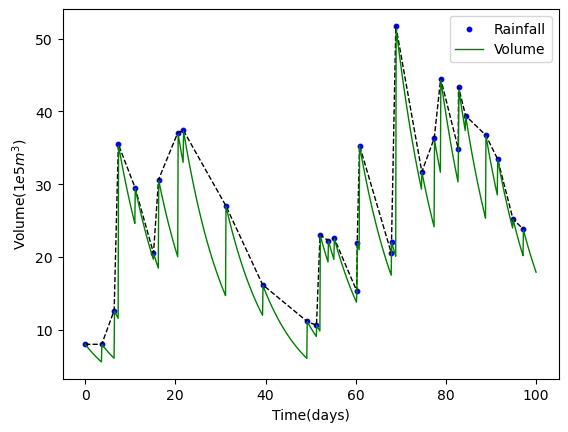
\includegraphics[width=0.7\textwidth]{rainfall.png}
  \caption{Une simulation du volume d'eau pour $\lambda=0.3$, $b=0.5$, $\delta_1=0.07$, $\delta_2=0.7$, $r_i=0.1$, $x_0^i=8$ dans les unités de «jour» et «$10^5m^3$». La courbe verte représente l'évolution du volume au cours du temps. Les points bleue représente les volumes d'eau après chaque pluie.}
  \label{v_e}
\end{figure}

Une illustration des évolutions de volume d'eau est donnée dans le figure \ref{v_e}. Nous remarquons que nous pouvons obtenir deux types des données : les volumes d'eau après chaque pluie, qui a la même longeur que les chutes de pluie, et les volumes d'eau au cours de temps. En général, le premier type de donnée est suffisant, car nous considérons principalement le rique d'inondation.

\section{Risque d'inondation}
Dans cette section, nous allons introduire de différentes approches pour simuler le rique d'inondation. Pour un premier temps, nous considérons le cas d'un seul barrage. Nous utilisons les notations sans indice $i$ comme $X_t$ et $A_t$. et nous formulons le problème de rique d'inondation comme suit : nous voulons trouver le seuil $x^\ast$ (soit pour un certain $T$, on prend $X=X_T$, soit pour le volume maximum dans $[0,T]$, on prend $X=\max_{0\le s\le T}X_s$) tel que
\[\mathbb{P}(X>x^\ast)\leq \alpha.\]
\paragraph{Monte-Carlo naïf} La méthode de Monte-Carlo naïf pour trouver un quantile $1-\alpha$ est de simuler $N$ trajectoires de $X$, notons $(X_i)$ et de prendre le quantile empirique. Nous rappelons que le quantile empirique est donné par
\[\hat{q}_{1-\alpha} = \inf\{x\in \mathbb{R}:\hat{F}_N(x)\geq 1-\alpha\},\]
où $\hat{F}_N$ est la fonction de répartition empirique. 
\[ \hat{F}_N(x) = \frac{1}{N}\sum_{i=1}^N \mathbf{1}_{X_i\leq x}.\]
Si nous trions les valeurs de $X_i$ comme $X_{(1,N)}\leq X_{(2,N)}\leq \cdots \leq X_{(N<N)}$, alors nous avons
\[\hat{q}_{1-\alpha} = X_{(\lceil N(1-\alpha)\rceil,N)}.\]
\paragraph{Importance Sampling} L'idée de l'importance sampling dans la contexte d'estimation de quantile, comme décrit dans l'article de Glynn\footnote{Glynn, Peter W. "Importance sampling for Monte Carlo estimation of quantiles." }, est de changer la mesure de probabilité vers une loi qui est plus «dense» dans la région de quantile. Ici pour le processus de Poisson composé $A_t=\sum_{i=1}^{N_t}U_i$ de paramètres $(\lambda, \nu)$, nous utilisons une transformation de Esscher, i.e. pour une fonction $f$ mesurable t.q. $\E[\exp(f(U))]<\infty$, nous avons pour toute $g$ mesurable bornée,
\[\E[g(A_t)]=\E_f\left[g(A_t)\exp\left((\lambda_f-\lambda)T-\sum_{i=1}^{N_t}f(U_i)\right)\right],\]
où $\lambda_f = \lambda \E[e^{f(U)}]$ et $\displaystyle \nu_f(du)=\frac{e^{f(u)}\nu(du)}{\E[e^{f(U)}]}$. Un estimateur de type Monte-Carlo pour $\E[g(A_t)]$ est donné à l'aide d'un échantillon $(A_t^{(i)})$ du processus de Poisson composé sous la mesure $(\lambda_f,\nu_f)$,
\[\E[g(A_t)]\approx \exp((\lambda_f-\lambda)T) \frac{1}{M}\sum_{i=1}^M g(A_t^{(i)})\exp\left(-\sum_{i=1}^{N_t^{(i)}}f(U_i^{(i)})\right).\]
Si nous voulons estimer un quantile $\alpha$, on peut prendre $g(x)=\mathbf{1}_{X(A_t)>x^\ast}$, où $X(A_t)=\max_{0\le s\le T}X_s(A_t)$ ou $X(A_t)=X_T(A_t)$ pour les deux cas. Et nous espérons de trouver $x^\ast$ t.q. $\E[g(A_t)]=\alpha$. Un algorithme pour estimer $x^\ast$ est de trier les valeurs de $X(A_t^{(i)})$ et de prendre le quantile empirique. Plus précisément, nous pouvons trouver l'indice $k_\alpha$ t.q.
\[\sum_{i\ :\ X^{(i)}(A_t)\le X^{(k_\alpha)}(A_t)}\exp\left(-\sum_{i=1}^{N_t^{(i)}}f(U_i^{(i)})\right)\approx M\alpha\exp(-(\lambda_f-\lambda)T),\]
alors $X^{(k_\alpha)}(A_t)$ est une estimation de $x^\ast$. En général, nous ne souhaitons pas que $k_\alpha$ soit trop proche de $M$ ou $1$, et c'est pourquoi nous effectuons un algorithme de l'importance sampling.

Un choix candidat (voir Annexe A pour plus de détails) pour $f$ est $f(u)=\sigma u$, où $\sigma$ est racine de l'équation
\[-\sigma \phi_A'(\sigma)+\phi_A(\sigma)=\log(\alpha),\]
où
\[\phi_A(\sigma)=\lambda T(M_U(\sigma)-1),\ M_U(\sigma)=b\frac{\delta_1}{\delta_1-\sigma}+(1-b)\frac{\delta_2}{\delta_2-\sigma}.\]
Dans le pratique, on peut résoudre cette équation facilement par la méthode numérique, car $\sigma\mapsto -\sigma \phi_A'(\sigma)+\phi_A(\sigma)$ est typiquement une fonction strictement décroissante.
\paragraph{Algorithme de la dernière particule}

L'idée de l'algorithme de la dernière particule est de renouveler la valeur minimale d'une suite de $X$ selon la loi de $(X|X>L)$ où $L=\min(X_i)$. 

Précisément, on simule d'abord une suite, notons $(X_i)_{1\leq i\leq n}$, selon la loi de $X$. On note le minimun temporaire $L=\min_{1\leq i\leq n}(X_i)$, et on remet à jour ces $X_i$ égaux à $L$ par un échantillon indépendant selon la loi de $(X|X>L)$. En répétant ce processus $\displaystyle \left\lceil\frac{\log \alpha}{\log(1-1/n)}\right\rceil$ fois, le minimum final $L$ est le seuil dont on a besoin.

Il nous reste à obtenir un échatillon selon la loi de $(X|X>L)$. Rappelons que $X_t$ est obtenu du processus de Poisson composé $A_t$, d'où il suffit de mettre à jour $A_t$ correspondant. L'idée est à partir d'une autre particule, on fait quelques itérations pour que ce soit presque indépendent de celle originale. Pour ce faire, on utilise l'algorithme de coloriage pour renouveler $N_t$ et pour des $U_i$, on obtient une combinaison des valeurs originales et des échantillons indépendants si le $i$-ième saut est gradé, où la proportion $q$ sera considérée dans la partie numérique. La possibilité de grader des points de saut $p$ sera aussi analysée dans la partie numérique. Le nombre d'itérations $M$ n'est pas forcément fixé, ce qui va jouer un rôle important dans la pratique.



\section{Simulation numérique} 
Dans cette section, nous allons appliquer ces approches dans un contexte réel. Nous déterminons d'abord les paramètres phisiques, et puis testons ces trois approches pour un $\alpha$ pas très petit de sorte que nous pouvons comparer ses performance. En fin nous essayons de trouver les estimations du quantile de $1-10^{-6}$ en utilisant l'importance sampling et l'algorithme de la derinière particule.


\paragraph{Paramètres physiques} On met l'unité de temps comme $1$ an et l'unité de volume comme $10^5m^3$. On a que $r^i=1$ et $T=1$. On suppose qu'il pleut $\lambda=70$ fois par an. On fixe en plus $\delta_1=0.07$ et $\delta_2=0.7$, où son unité est $(10^5m^3)^{-1}$ et l'inverse de $\delta_i$ montre le volume moyen d'une seule pluie. Le quantile $\alpha$ considéré est $10^{-6}$, et on prend la proportion $b=0.1$, i.e. seule une sur dix est une grande pluie.

Maintenant on va considérer la valeur de $x_0$, le volume initial. On veut que $x_0$ soit <<l'état stationnaire>> pour que ce soit compatible avec le processus physique, i.e. le flux d'eau entrant et sortant est presque équilibré pendant assez longtemps. Dans la pratique, on simule $5,000$ fois $X_{100}$ et puis calcule le moyen, cela nous donne $x_0=190$.

Cette idée peut aussi être réalisée par un calcul théorique. Pour un petit temps $\Delta t$, le flux sortant est $-(r_1 x_0)\Delta t$ alors que le flux entrant est $\mathbb E[\nu](\lambda_1\Delta t)$. Pour que $x_0$ soit l'état stationnaire, on a forcément que  $-r_1x_0+\lambda_1{\mathbb E[\nu]}=0$, d'où
\[x_0=\frac{\lambda_1}{r_1}\left(\frac{b}{\delta_1}+\frac{1-b}{\delta_2}\right)=190.\]

\paragraph{Variantes de l'algorithme de la dernière particule} On a trois manières d'implémenter cet algorithme, avec de petites différences entre eux. Le point clé est que, lorsque $\alpha$ est petit, l'algorithme peut s'arrêter parce que toutes les particules prennent la même valeur. Ainsi, afin d'obtenir un échatillon selon la loi de $(X|X>L)$, il nous faut considérer le nombre d'acceptions $\tilde M$ au lieu du nombre d'itérations $M$. 

On a alors deux approches pour augmenter le nombre d'acceptions, en voyant qu'il est $M$ multiplié par le taux d'acceptions. On peut augmenter directement le nombre, soit $M$ va croître pendant l'algorithme, soit l'algorithme ne s'arrête qu'après avoir obtenu un certain nombre d'acceptations, i.e. $\texttt{while}$ au lieu de $\texttt{for}$. On peut également améliorer le taux d'acceptation, en changeant $q$ et $p$. Il convient de souligner que les valeurs de $p$ et $q$ dépendent en fait de $\alpha$. On intrduit alors deux manières d'implémenter cet algorithme, l'un est avec $M$ croissant et l'autre demande que le nombre d'acceptations $\tilde M$ est au moins $M/2$, où ces $p$ et $q$ ne sont en vrai pas forcément pareils. La discussion détaillée se trouvera à l’Annexe B.

\paragraph{Comparison des trois approches pour $\alpha=10^{-2}$} Nous pouvons imaginer que, pour $\alpha$ n'est pas très petit, nous allons trouver un correspondance entre les trois approches. Plus précisement, nous utilisons un algorithme de Monte-Carlo naïf pour $N=10,000$, un algorithme de l'importance sampling pour $N=10,000$ et $f(x)=0.031x$, un algorithme de la dernière particule avec $M$ croissant pour $N=1,000$, $M_0=20$. Les résultats sont montrés dans la figure \ref{0.1} : les trois algorithmes donnent le même résultat, tandis que l'importance sampling a une variance plus petite. Nous remarquons aussi que l'algorithme de la dernière particule nous permet aussi d'obtenir une estimation pour la distribution après la volume critique $x^\ast$ : $p(x|x>x^\ast)$, comme montré dans la figure \ref{0.2}.
\begin{figure}[H]
    \centering
    \includegraphics[width=0.8\textwidth]{1-1.png}
    \caption{Estimation du quantile de 0.99 par les trois méthodes. 10 expériences indépendants sont faits pour chaque méthode. Ici nous représentons l'erreur comme $(\max - \min)$.}
    \label{0.1}
\end{figure}
\begin{figure}[H]
    \centering
    \includegraphics[width=0.8\textwidth]{1-2.png}
    \caption{Estimation de la distribution $p(x|x>x^\ast)$ pour $\alpha=0.01$.}
    \label{0.2}
\end{figure}
\paragraph{Résultat final pour $\alpha=10^{-6}$} Quand $\alpha$ est maintenant $10^{-6}$, on peut imaginer que, l'algorithme de Monte-Carlo naïf ne marche plus dans ce cas, ces résultats seront hautement aléatoires. Malgré tout, l'algorithme de l'importance sampling pour $N=10,000$ et un algorithme de la dernière particule avec le nombre d'acceptations $\tilde M=15=M/2$ nous donnent deux résultats assez proches, ce qui montre l'efficacité de ces deux algorithmes lorsque $\alpha$ est extrêmement petit, vu dans la figure \ref{0.3}.
\begin{figure}[H]
    \centering
    \includegraphics[width=0.8\textwidth]{output 0.000001.png}
    \caption{Estimation du quantile de 0.999999 par les trois méthodes. 10 expériences indépendants sont faits pour chaque méthode. Ici nous représentons l'erreur comme $(\max - \min)$.}
    \label{0.3}
\end{figure}
On remarque que les valeurs de l'algorithme de la dernière particule sont globalement un peu plus élevées, ce qui peut s'expliquer par le fait que, dans cet algorithme, les valeurs des particules ne sont pas totalement indépendantes lors de leur itération, car elles proviennent d'une chaîne de Markov qui s'écarte des autres particules ayant des valeurs plus élevées, et qui ont donc tendance à être plus grandes.
\section{Conclusion}
Nous avons réussi à simuler le risque d'inondation, qui est un effet un événement rare, avec deux approches différentes : l'importance sampling et l'algorithme de la dernière particule. En général, l'importance sampling est très efficace pour ce problème et donne un résultat assez précis, tandis que l'algorithme de la dernière particule est plus flexible et nous permet aussi d'estimer la distribution après le niveau critique. Le choix de paramètre dans importance sampling et les choix des hyperparamètres dans l'algorithme de la dernière particule jouent un rôle très important dans la simulation numérique. Les études sur ces facteurs sont donc crucial pour ce type de problème.
\paragraph{Travaux de future} Nous avons encore de points à améliorer dans ce problème, par example : 
\begin{itemize}
    \item Prise en compte l'impact de $\beta$ dans l'importance sampling. Nous avons utilisé un transformation de $f(x)=\sigma x+\beta$ avec $\beta =0$. En fait, prendre un $\beta>0$ a un impact similaire que prendre $\sigma>0$. En jouant en même temps avec $\sigma$ et $\beta$, nous avons la possibilité  d'obtenir une variance plus petite.
    \item Quant à l'algorithme de la dernière particule, on n'a toujours pas assez bien compris les relations entre de nombreux paramètres quantitativement et profondément, car on a encore utilisé des méthodes numérique pour montrer ce type de relations. En fait, il est possible d'analyser et d'optimiser ces paramètres de manière plus théorique afin de trouver les meilleures valeurs possibles. En outre, afin de mieux comprendre la relation entre des paramètres tels que $p$ et $q$, l'analyse multidimensionnelle, qui consiste par exemple à prendre $(p,q)\in [0,1]^2$ pour dessiner un graphique tridimensionnel à analyser, est également une direction qui peut être élargie.
\end{itemize}
% Conclusion and perspective

\newpage
\section*{Annexe A : choix du coefficient dans l'importance sampling}
Dans le contexte d'estimation Monte-Carlo du quantile, Glynn\footnote{P. W. Glynn "Importance Sampling for Monte Carlo Estimation of Quantiles"} suggère un choix possible pour le changement de loi. L'idée est basée sur une tail approximation 
\[\P(X>x)\approx \exp(-x\theta_x+\phi(\theta_x)),\]
où $\phi(s)=\log\E[\exp(sX)]$ est la fonction génératrice des cumulants, $\theta_x$ est la racine d'équation $\phi'(\theta_x)=x$. En particulier, pour $\alpha$ un niveau donné, soit $\theta_\alpha$ la solution de
\begin{equation}
\label{eq}
    -\theta_\alpha \phi'(\theta_\alpha)+\phi(\theta_\alpha)=\log \alpha,
\end{equation}
nous avons
\[\P(X>\phi'(\theta_\alpha))\approx \alpha,\]
donc $\phi'(\theta_\alpha)$ peut être considéré comme l'estimateur du quantile de $1-\alpha$. En général cette approximation sera grossière, nous considérons donc un changement de la loi $\tilde{F}(dx)=\exp(\theta_\alpha x-\phi(\theta_\alpha))F(dx)$, ce qui conduit une loi de moyenne $\phi'(\theta_\alpha)$ :
\[\tilde{\E}[X]=\int x\exp(\theta_\alpha x-\phi(\theta_\alpha))F(dx)=\frac{\E[X\exp(\theta_\alpha X)]}{\exp \phi(\theta_\alpha)}=\frac{\partial }{\partial s}(\log\E[\exp(sX)])\biggr|_{\theta_\alpha},\]
ce qui indique donc que, sous $\tilde{F}$, l'échantillonnage à partir de l'événement associé au quantile $1-\alpha$ n'est plus un événement rare. En fait, comme la fonction génératrice de moment détermine complètement la loi, nous pouvons caractériser cette transformation par 
\begin{equation}
\label{1}
\begin{split}
 \tilde{\phi}(s)&=\log\tilde{\E}[e^{sX}]=\log\int e^{sx}e^{\theta_\alpha x-\phi(\theta_\alpha)}F(dx)=\log\left(\frac{\E[e^{(s+\theta_\alpha)X}]}{e^{\phi({\theta_\alpha})}}\right)\\
 &=\phi(s+\theta_\alpha)-\phi(\theta_\alpha).
\end{split}
\end{equation}
Pour notre modèle du processus de Poisson composé $(\lambda,\nu)$, le changement de loi est réalisé par la transformation de Esscher, i.e. à partir d'une $f$ mesurable bornée, nous obtenons un nouveau processus de Poisson composé de paramètres $(\lambda_f,\nu_f)$ 
où $\lambda_f = \lambda \E[e^{f(U)}]$ et $\displaystyle\nu_f(du)=\frac{e^{f(u)}\nu(du)}{\E[e^{f(U)}]}$. Si nous supposons que $f$ est linéaire : $f(x)=\sigma x+\beta$, nous pouvons également caractériser cette transformation par les cumulants :
\[\phi(s)=\lambda t(\E[e^{sX}]-1),\]
et
\begin{equation}
\label{2}
    \begin{split}
    \tilde{\phi}(s)&=\lambda_ft(\E_f[e^{sX}]-1)=\lambda t\E[e^{\sigma X}]e^{\beta}\left(\frac{\E[e^{(s+\sigma)X}]}{\E[e^{\sigma X}]}-1\right)\\
    &=\lambda te^{\beta}(\E[e^{(s+\sigma)X}]-\E[e^{\sigma X}])\\
    &=e^{\beta}(\phi(s+\sigma)-\phi(\sigma)).
\end{split}
\end{equation}
Donc si nous posons $\beta=0$, l'équation (\ref{2}) aura la même forme que l'équation (\ref{1}), la technique de Glynn s'applique pour notre processus de Poisson. Pour conclure, un choix possible pour $f$ est $f(x)=\sigma x$, où $\sigma$ satisfait la condition de (\ref{eq}), i.e.
\[-\sigma \phi_A'(\sigma)+\phi_A(\sigma)=\log(\alpha),\]
où
\[\phi_A(\sigma)=\lambda T(M_U(\sigma)-1),\ M_U(\sigma)=b\frac{\delta_1}{\delta_1-\sigma}+(1-b)\frac{\delta_2}{\delta_2-\sigma}.\]
\section*{Annexe B : choix des parametères dans l'algorithme de la dernière particule}
Dans la pratique, sauf les paramètres physiques, on a encore le nombre de particules $N$, le nombre d'itérations $M$, la probabilité de grader des points de saut $p$ et la proportion de valeurs originales $q$, à déterminer. On considère deux côtés : l'exactitude et l'efficacité.

Pour $N$ nombre de particules, le plus grand est $N$, le résultat est généralement plus précis, alors que la complexité temporelle est 
\[O(N\cdot\frac{1}{\log(1-1/N)})=O(N^2),\]
quand $N$ est grand, d'où on choisit ici $N=1000$.

Avant de commencer la discussion suivante sur d'autres paramètres, on aimerait montrer la figures \ref{0.5} pour illustrer la possibilité que, mentionné dans le texte principal, l'algorithme s'arrête à une valeur égale pour toutes les particules. 

\begin{figure}[H]
    \centering
    \includegraphics[width=0.8\textwidth]{output iteration}
    \caption{Pour différents $p\in[0.1,0.6]$, tracer le taux d'acceptations pour chaque appel à $\texttt{get\_new\_rainfall}$, où $\alpha=0.01$ est fixé.}
    \label{0.5}
\end{figure}

On voit qu'aussi que soit le $p$, même pour $\alpha=0.01$ pas si petit, il peut toujours y avoir en moyen $30\%$ des itérations avec des taux d'acceptations inférieurs à $15\%$. Cela signifie que le risque d'échec de cet algorithme est élevé, mais aussi nous donne la motivation et la nécessité d'étudier d'autres paramètres.

% La relation entre $p$ et $M$ sera compliquée. On analyse d'abord séparément ces deux paramètres. 
Pour $M$, il semble que c'est toujours mieux que $M$ soit grand, puisque plus grand est le nombre d'itérations, le résultat est plus indépendent de celui original. Mais, on ne peut pas prendre $M$ arbitairement grand en considérant l'éfficacité. On examine donc $p$, qui est déjà pas facile, mais nous aide à obtenir l'éfficacité sans perdre trop d'exactitude.

Lorsque $p$ devient grand, le résultat peut avoir deux effets. D'une part, cela rend chaque itération de $\texttt{get\_new\_rainfall}$ plus indépendante, puisqu'il y a plus de nouveaux points générés aléatoirement de manière indépendante ; d'autre part, c'est précisément le fait qu'il y ait tant de nouveaux points qui tend à entraîner des valeurs $\texttt{L}$ correspondantes très basses, et donc une probabilité de rejet plus élevée. Pour que les résultats soient précis, $p$ doit être aussi petit que possible ; pour améliorer l'efficacité, en particulier le taux d'acceptations, $p$ ne doit pas être trop petit.

En fixant $p$, deux approches ont des effets similaires : l'une qui augmente progressivement $M$ au fil des itérations et l'autre qui passe directement d'un nombre fixe d'itérations à un nombre fixe d'acceptations $\tilde M$. En supposant qu'après un certain nombre d'acceptations, il peut être considéré comme indépendant, nous avons choisi d'analyser davantage ce dernier, c'est-à-dire de fixer $\tilde M=M/2=15$ pour changer $p$ afin de trouver un meilleur $p$.

\begin{figure}[H]
    \centering
    \includegraphics[width=0.71\textwidth]{output p ++ 0.1.png}
    \caption{Pour différents $p\in[0.1,0.9]$, comparer les résultats de l'algorithme de la dernière particule avec ceux de Monte Carlo naïf représentés par les lignes horizontales rouges, où $\alpha=0.01$ est fixé.}
    \label{0.4}
\end{figure}

D'où, selon la figure \ref{0.4}, on constate que l'intervalle $[0.1, 0.8]$ est un intervalle possible pour $p$. À l'avenir, pour l'efficacité de l'algorithme puis gagner du temps, mais aussi pour l'exactitude, on aura tendance à choisir $p$ autour de $0.4$. Ainsi, un tel $p$ peut garantir une certaine validité même lorsque $\alpha$ devient petit.

Puisque $q$ provient de l'optimisation de la matrice de transition dans Metropolis-Hastings. Lorsque $q = 1$, il est simple de conserver toutes les valeurs prises à l'origine, et lorsque $q = 0$, c'est de reprendre toutes les valeurs, les deux satisfaisant Metropolis-Hastings, mais un mélange des deux sera en fait compliqué. 

 D'un point de vue théorique, lorsque $p$ est petit, cela signifie qu'on a tendance à choisir de nouveaux points de saut et que, par conséquent, on peut avoir tendance à préserver les anciennes valeurs dans les points de saut préservés, c'est-à-dire que $q$ est relativement grand. Si $p$ et $q$ sont tous petits, on revient complètement à Monte Carlo naïf, tandis que si $p$ et $q$ sont tous grands, il est difficile d'obtenir une véritable indépendance dans $\texttt{get\_new\_rainfall}$, et de conduire à un résultat inexact.

Cependant, en général, plus $q$ est grand, plus les valeurs aux points de saut originaux sont préservées, et plus sa valeur $\texttt{L}$ est grande, plus il est facile d'accepter et plus il est efficace. On montre maintenant la figure \ref{0.6} qui représente les résultats comparés avec l'algorithme de Monte-Carlo naïf quand $q$ varie, en fixant $\alpha=0.01$ et $\tilde M=15$, où encore, les effets indirects des autres paramètres sont réduits en fixant $\tilde M$.

\begin{figure}[H]
    \centering
    \includegraphics[width=0.8\textwidth]{output q 0.01.png}
    \caption{Pour différents $q\in[0.1,0.9]$, comparer les résultats de l'algorithme de la dernière particule avec ceux de Monte Carlo naïf représentés par les lignes horizontales rouges, où $\alpha=0.01$ est fixé.}
    \label{0.6}
\end{figure}

Ainsi, on peut prendre ici par exemple $q=0.9$ raisonnablement, i.e. en fixant le nombre d'acceptations, on peut toujours prendre $q$ grand en ignorant ses aspects négatifs (sans indépendence).


\end{document}


